\documentclass
[answers]
{exam}

\linespread{1.1}

\usepackage{amsmath, amssymb, amsthm}  %% 數學符號用txfonts
\usepackage{mathrsfs} 
%\usepackage{pstricks,pstricks-add} % 引入 pstricks 和 pstricks-add 套件 (繪圖套件) 
%插入GGB圖片===================================
\usepackage{pgf,tikz}
\usepackage{mathrsfs}
\usetikzlibrary{arrows}
%=============================================
\usepackage{graphicx}   %% 插入圖片用
\usepackage{float}  %%強制插入圖片位置
\usepackage{caption}
\usepackage{subfigure}
\usepackage{color}
%\usepackage{minitoc}   %chapter下的小目錄
\usepackage{colortbl}
\usepackage{nopageno}
\usepackage{cases}
\usepackage{textcomp}             % for \textcelsius
\renewcommand{\arraystretch}{1.2} % 將表格行間距加大為原來的 1.2 倍
\arrayrulewidth=1pt               % 調整線條粗細為 1pt
\tabcolsep=15pt                   % 調整欄間距為 24pt


%\begin{figure}[h]
%\includegraphics[scale=1.2]{./figure/2.png}
%\end{figure}

\usepackage{wrapfig}  %%圖文並排

%\begin{wrapfigure}{r}{6cm}  r:圖片靠右  6cm:離右邊6cm
%	\centering  圖片在右邊區塊的中間
%	\includegraphics[scale=0.6]{./figure/19.png}
%\end{wrapfigure}

\usepackage{tcolorbox}  %% 顏色方框
\usepackage{tikz}  %%繪製流程圖、腦圖...
\usepackage{array}  %%陣列
\usepackage{booktabs} %調整表格線與上下內容的間隔
\usepackage{multirow}
\usepackage{enumitem}
%可改enumerate的label
\usepackage{tasks}  %%選擇題
\settasks{label=(\Alph*),
		  label-width=3.5ex,
		  label-offset={0.4em},
		  label-align=left,
		  column-sep={1pt},
		  item-indent={21pt}, %%選項前後
		  before-skip={-0.7em},
		  after-skip={-0.7em}}
%[label=(\Alph*),label-width=4ex]  
%\Alph* 選項ABCD  \alph* 選項abcd  \arabic* 選項1234 \roman*羅馬數字
\usepackage{framed}  %%框框
%出入單行字加框  \framebox[\width]{我是一段话}

%插入圖片 \rightline{\includegraphics[scale=1.2]{./chapter_1/figure/1.png}}
\usepackage{diagbox}  %%斜線表格頭
\usepackage{ulem}
%\sout{文字} 刪除線		\uwave{文字} 波浪線
%\xout{文字} 斜刪除線		\uuline{文字} 雙下划線
\usepackage[margin=2cm]{geometry} %邊界設定
\usepackage[export]{adjustbox} %插入圖片
\usepackage[colorlinks=true,linkcolor=blue]{hyperref}
%%[是否開啟目錄顏色,目錄顏色設定]{超連結}

%\usepackage{fancyhdr}  %%這兩行是頁首頁尾
%\pagestyle{fancy}  %%頁首頁尾格式
%\fancypagestyle{plain}{}
%\renewcommand{\headrulewidth}{0.4pt}  %%頁首下方直線厚度
%\cfoot{觀念解數學--~\thepage~--態度解人生}
%\fancyhead{} % 清除所有頁首設定
%\fancyhead[RO,LE]{\thechapter}
%\fancyfoot{} % 清除所有頁尾設定
%\fancyfoot[LE,RO]{第~\thepage~頁}      % 頁碼放在偶數頁的左邊及奇數頁的右邊
%\fancyfoot[LO,CE]{奇數頁左及偶數頁中}
%\fancyfoot[CO,RE]{奇數頁中及偶數頁右}
% Texmaker使用者: 上方選擇XeLaTeX後再編譯
\usepackage{xeCJK}   % Chinese input settings
\setCJKmainfont{標楷體} % Windows使用者請使用這行
\setmainfont{Times New Roman}
\defaultCJKfontfeatures{AutoFakeBold=0.5,AutoFakeSlant=0} %以後不用再設定粗斜
\newCJKfontfamily\WC{華康行楷體W5}                       
\XeTeXlinebreaklocale "zh"
\XeTeXlinebreakskip = 0pt plus 1pt
%%上兩行才能讓中文自動換行
\makeatletter
\def\rightharpoonfill@{\arrowfill@\relbar\relbar\rightharpoonup}
\newcommand{\vect}{\mathpalette{\overarrow@\rightharpoonfill@}}
\makeatother
%向量

%\renewcommand{\qedsymbol}{}
\newcommand{\R}{\mathbb{R}} %mathbb 雙行粗體
\newcommand{\Z}{\mathbb{Z}}
\newcommand{\Q}{\mathbb{Q}}
\newcommand{\N}{\mathbb{N}}
\renewcommand{\S}{\mathbb{S}}
\newcommand{\f}{\ensuremath{\mathcal{F}}} 
%%\ensuremath  非數學模式自動加上$符號
\newcommand\norm[1]{\left\lVert#1\right\rVert}
\newcommand\abs[1]{\left| #1\right| }
\newcommand\ul[1]{\uline{\hspace*{#1}}}
\newcommand\px{\kern 0.56em/\kern -0.8em /\kern 0.56em}
%文繞圖 wrapfigure 和 條列式環境 item 並列, 需在 enumerate 環境之中
%\itemwrap{<先用 \begin{wrapfigure} 環境插入圖片, 再接著文字>}
\newcommand{\itemwrap}[1]{
	\item \parbox[t]{\dimexpr\textwidth-\leftmargin}{
		\vspace{-3.2mm}#1}}

%\itemwraps{<需縮排的行數>}{<圖片寬度(配合上面寬度)>}{<文字>}
\newcommand{\itemwraps}[3]{
	\item \parbox[t]{\dimexpr\textwidth-\leftmargin}{%
		\vspace{-3.2mm}
		\begin{wrapfigure}[#1]{r}{#2}
		\end{wrapfigure}#3}}


\newif\ifqr\qrfalse %QR
\newcommand{\qr}[1]{\ifqr\relax\else #1\fi} 
%教用學生版 %一鍵隱藏答案  \true隱藏  \false顯示

\newif\ifans\ansfalse
\newcommand{\ans}[1]{\ifans\relax\else\framebox{#1}\fi} 

\DeclareMathOperator{\sign}{sign} %sign為非斜體

\parindent=0pt  %%首行空格
\renewcommand{\qedsymbol}{}  %證明後面沒方格

%\theoremstyle{remark}
%\newtheorem{prop}{Proposition}
%\newtheorem{thm}[prop]{Theorem}   %% 編號跟著 prop 走
%\newtheorem*{thm}{Theorem}   %% 有自己的編號
%\newtheorem{lem}{\underline{Lemma}}
%\newtheorem*{rmk}{\bf{\underline{Remark}}}
%\newtheorem*{ex}{\underline{Examples}}
%\newtheorem{cor}{Corollary}
%\newtheorem*{coro}{Corollary}
%\newtheorem{lem}[thm]{Lemma}
\theoremstyle{definition}
%\newtheorem*{defn}{Definition}
\newtheorem{foc}{\WC\underline{\Large{焦點}}}[section]
\newtheorem*{pra}{\WC\underline{\Large{隨堂小練}}}
\newtheorem*{hw}{\WC\underline{\Large{課後練功坊}}}
\newtheorem*{suyu}{\WC\underline{\Large{素養挑戰題}}}

\newif\ifyr\yrfalse %年分
\newcommand{\yr}[1]{\ifyr\relax\else #1\fi} 
%教用學生版 %一鍵隱藏答案  \true隱藏  \false顯示

\newif\ifsho\shofalse %學校
\newcommand{\sho}[1]{\ifsho\relax\else\rightline{【#1】}\fi} 
%教用學生版 %一鍵隱藏答案  \true隱藏  \false顯示

\newif\ifpos\posfalse %編號
\newcommand{\pos}[1]{\ifpos\relax\else\framebox{位置:#1}\fi} 
%教用學生版 %一鍵隱藏答案  \true隱藏  \false顯示

\newif\ifno\nofalse %編號
\newcommand{\no}[1]{\ifno\relax\else\framebox{編號:#1}\fi} 
%教用學生版 %一鍵隱藏答案  \true隱藏  \false顯示

\newif\ifvn\vnfalse %空行
\newcommand{\vn}[1]{\ifvn\relax\else #1\fi}

\usetikzlibrary{shapes.geometric}
\newcommand{\Stars}[2][fill=black,draw=black]{\begin{tikzpicture}[baseline=-0.35em,#1]
\foreach \X in {1,...,3}
{\pgfmathsetmacro{\xfill}{min(1,max(1+#2-\X,0))}
\path (\X*1.1em,0) 
node[star,draw,star point height=0.25em,minimum size=1em,inner sep=0pt,
path picture={\fill (path picture bounding box.south west) 
rectangle  ([xshift=\xfill*1em]path picture bounding box.north west);}]{};
}
\end{tikzpicture}}


%有*是無編號  無*是有編號
% Authur information
%\title{標題}
%\author{作者}
%\date{日期}

%\begin{document}
%\renewcommand{\qedsymbol}{}  %證明後面沒方格
%\maketitle   %此功能為是否顯示title
%\fontsize{20pt}{25pt}\selectfont  %%目錄字體大小
%\tableofcontents  %%目錄

%\fontsize{12pt}{25pt}\selectfon


%===================================================================

\title{{\Huge{\WC{A}}}}
\author{}
\date{}

\begin{document}

%\fontsize{20pt}{25pt}\selectfont  %%目錄字體大小
%\tableofcontents  %目錄
\let\cleardoublepage\clearpage
\fontsize{12pt}{25pt}\selectfont  %%內文字體大小
\newpage
%-----------------------------------------------------
\maketitle
%\section{\WC{直線方程式}}
%\subsection{~}
%\subsubsection{直角坐標與斜率}

\begin{questions}


%1
\question
下列何者是最簡根式?
\begin{tasks}(4)
	\task $\sqrt{75}$
	\task $\dfrac{2}{9}\sqrt{7}$
	\task $\dfrac{3}{\sqrt{6}}$
	\task $\sqrt{\dfrac{5}{19}}$
\end{tasks}
\begin{solution}~\\
	B
\end{solution}
%\sho{\yr{104}全模 2}


%2
\question
已知$3x^2 + 5x -2 =(3x-1)(x+2)$,則下列式子是$3x^2+5x-2$的因式有幾個?
\begin{tasks}(3)
	\task[(甲)] \ $-3x+1$
	\task[(乙)] \ $x-\dfrac{1}{3}$
	\task[(丙)] \ $3x^2+5x-2$
	\task[(丁)] \ $x-2$
	\task[(戊)] \ $9x^2+15x+6$
	\task[(己)] \ $x+2$
\end{tasks}
\begin{tasks}(4)
	\task 6個
	\task 5個
	\task 4個
	\task 3個
\end{tasks}
\begin{solution}~\\
	C
\end{solution}

%3
\question
將 $16x^2-ax+25$ 因式分解,可得$(4x-b)^2$ 的形式,若 $b$ 為負整數,則 $2a-3b$ =?
\begin{tasks}(4)
	\task -65
	\task 65
	\task 95
	\task -95
\end{tasks}
\begin{solution}~\\
	A
\end{solution}

%4
\question
小明想要將$\dfrac{1}{\sqrt{28}+\sqrt{7}}$ 的分母有理化,則分子、分母同乘以下列哪一個選項中的數值是無法辦到的?
\begin{tasks}(4)
	\task $\sqrt{28}\times\sqrt{7}$
	\task $\sqrt{7}$
	\task $\sqrt{28}+\sqrt{7}$
	\task $\sqrt{28}-\sqrt{7}$
\end{tasks}
\begin{solution}~\\
	A
\end{solution}


%5
\question
設a、b均為正整數,且$25a^2-4b^2=29$,求a-b =?

\begin{tasks}(4)
	\task $4$
	\task $3$
	\task $-3$
	\task $-4$
\end{tasks}

\begin{solution}~\\
	D
\end{solution}

%6

\begin{minipage}[t]{0.7\linewidth}

\question
如右圖,有甲、乙、丙、丁四種類型的四邊形,其中有2個甲,1 個乙,2個丙,1個丁。今將這6個四邊形,拼成一個大的長方形,則其兩鄰邊的邊長分別為多少?
\begin{tasks}(4)
	\task $2x+1,x+b$
	\task $2x+b,x+1$
	\task $x+2b,2x+1$
	\task $x+1,2x+2b$
\end{tasks}


\end{minipage}
\hfill
\begin{minipage}[t]{0.3\linewidth}
\vspace*{-0.3cm}
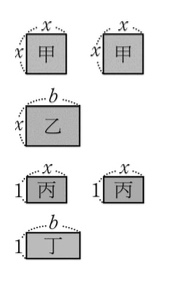
\includegraphics[scale=0.5]{./figure/A_1.jpg}
\raggedleft %靠右對齊
\end{minipage}

\begin{solution}~\\
	B
\end{solution}
%7
\question
若3、4、x是直角三角形的三邊長,則x值為\ul{50pt}
\begin{solution}~\\
	$5$或$\sqrt{7}$
\end{solution}

%8
\question
已知坐標平面上P(2,-1)、Q(-6,5)兩點,求$\overline{PQ}$的長度為
\ul{50pt}
\begin{solution}~\\
	$10$
\end{solution}

%9
\begin{minipage}[t]{0.7\linewidth}

\question
右圖為一長方體,$\overline{AB}$=3公分,$\overline{AD}$=4公分,$\overline{AE}$=5公分,則 $\overline{AG}$的長度為
\ul{50pt}公分

\end{minipage}
\hfill
\begin{minipage}[t]{0.3\linewidth}
\vspace*{-0.3cm}
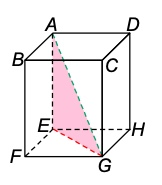
\includegraphics[scale=0.5]{./figure/A_2.jpg}
\raggedleft %靠右對齊
\end{minipage}


\begin{solution}~\\
	$5\sqrt{2}$
\end{solution}

%10
\question
一個直角三角形的兩股分別為5、12則此直角三角形斜邊上的高=
\ul{50pt}
\begin{solution}~\\
	$\dfrac{60}{13}$
\end{solution}

%11
\question
計算下列各式的值,並將結果化為最簡根式。
\begin{tasks}(1)
	\task $\dfrac{2}{\sqrt{3}}+\sqrt{12}-\sqrt{27}$ = \ul{50pt}\\
	\task $\sqrt{\dfrac{28}{25}}\times\sqrt{\dfrac{5}{14}}\div\left(-\sqrt{\dfrac{8}{5}}\right)$ = \ul{50pt}\\
	\task $\left(3\sqrt{7}+5\right)-3\div\left(\sqrt{7}-2\right)$= \ul{50pt}\\
\end{tasks}
\begin{solution}~\\
	(1)$-\dfrac{1}{3}\sqrt{3}$\\
	(2)$-\dfrac{1}{2}$\\
	(3)$2\sqrt{7}+3$
\end{solution}

%12
\question
因式分解下列各式:
\begin{tasks}(1)
	\task $2x^2-4x$ = \ul{50pt}
	\task $x^2-5x-bx+5b$ = \ul{50pt}
	\task $x^2+6x+9$ = \ul{50pt}
	\task $9x^2-y^2$ = \ul{50pt}
	\task $a^2-b^2-c^2+2bc$ = \ul{50pt}
	\task $\left(2x-1\right)\left(3x-7\right)-\left(1-2x\right)\left(7-3x\right)^2$ = \ul{50pt}
\end{tasks}
\begin{solution}~\\
	(1)$2x\left(x-2\right)$\\
	(2)$\left(x-b\right)\left(x-5\right)$\\
	(3)$\left(x+3\right)^2$\\
	(4)$\left(3x+y\right)\left(3x-y\right)$\\
	(5)$\left(a+b-c\right)\left(a-b+c\right)$\\
	(6)$\left(2x-1\right)\left(3x-7\right)\left(x-2\right)$
\end{solution}

%13

\begin{minipage}[t]{0.7\linewidth}

\question
如右圖,三角形ABC中,$\overline{AD}$垂直$\overline{BC}$於D點,E是$\overline{AD}$上任一點。已知$\overline{AB}$=13,$\overline{CE}$ =6,則$\overline{AC}^2+ \overline{BE}^2$=
\ul{50pt}

\end{minipage}
\hfill
\begin{minipage}[t]{0.3\linewidth}
\vspace*{-0.3cm}
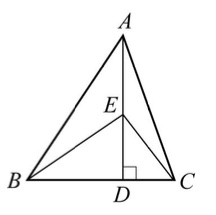
\includegraphics[scale=0.5]{./figure/A_3.jpg}
\raggedleft %靠右對齊
\end{minipage}


\begin{solution}~\\
	$205$
\end{solution}

%14
\question
計算$\dfrac{6}{\sqrt{5}+\sqrt{2}}+\dfrac{6}{\sqrt{8}+\sqrt{5}}+\dfrac{6}{\sqrt{11}+\sqrt{8}}+\dfrac{6}{\sqrt{14}+\sqrt{11}}+......+\dfrac{6}{\sqrt{50}+\sqrt{47}}$=
\ul{50pt}
\begin{solution}~\\
	$8\sqrt{2}$
\end{solution}

%15
\begin{minipage}[t]{0.7\linewidth}

\question
利用右邊乘方開方表,求$\sqrt{80}+\sqrt{0.4}$的近似值$\fallingdotseq$\ul{50pt}。 (四捨五入法取到小數點後第 2 位)

\end{minipage}
\hfill
\begin{minipage}[t]{0.3\linewidth}
\vspace*{-0.3cm}
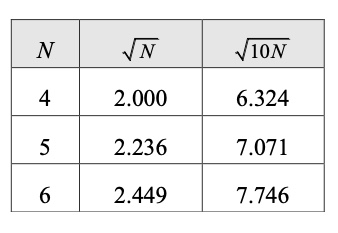
\includegraphics[scale=0.5]{./figure/A_4.jpg}
\raggedleft %靠右對齊
\end{minipage}

\begin{solution}~\\
	$9.58$
\end{solution}

%16
\begin{minipage}[t]{0.7\linewidth}

\question
在右圖的四邊形ABCD中,$\angle A=\angle C=90°$。若 $\overline{AB} =15$,$\overline{AD} =20$,$\overline{BC}=24$,則四邊形ABCD的周長為多少?

\end{minipage}
\hfill
\begin{minipage}[t]{0.3\linewidth}
\vspace*{-0.3cm}
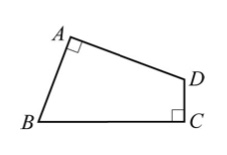
\includegraphics[scale=0.5]{./figure/A_5.jpg}
\raggedleft %靠右對齊
\end{minipage}

\begin{solution}~\\
	(1)$\overline{CD}=7$\\
	(2)$66$
\end{solution}

%17
\question
\begin{tasks}(1)
	\task 已知直角三角形的兩股長分別為1、6則斜邊長為多少?
	\task 已知$\triangle ABC$之三邊長為29、37、52 ,求$\triangle ABC$之面積?
\end{tasks}
\begin{solution}~\\
	(1)$\sqrt{37}$\\
	(2)16平方單位
\end{solution}

%\sho{\yr{104}全模 2}




\end{questions}

\end{document}
